\documentclass[11pt,a4paper]{article}

\usepackage[utf8]{inputenc}
\usepackage[T1]{fontenc}
\usepackage{lmodern}
\usepackage[margin=2.3cm]{geometry}
\usepackage{amsmath,amssymb}
\usepackage{booktabs,tabularx,array}
\usepackage{enumitem}
\usepackage{xcolor}
\usepackage{tikz}
\usetikzlibrary{arrows.meta,positioning,fit,backgrounds,calc}
\usepackage[hidelinks]{hyperref}
\usepackage{microtype}
\usepackage{parskip}
\usepackage{float}
\setlength{\emergencystretch}{4em}

\definecolor{accent}{RGB}{38,110,200}
\definecolor{soft}{RGB}{235,241,250}
\definecolor{warn}{RGB}{190,80,40}
\definecolor{grey}{RGB}{110,110,110}

\newcommand{\code}[1]{\texttt{#1}}
\newcommand{\term}[1]{\textbf{#1}}
\newcolumntype{L}{>{\raggedright\arraybackslash}X}

\newenvironment{keybox}[1]{%
  \par\smallskip\noindent\begin{tikzpicture}\node[draw=accent,fill=soft,rounded corners=3pt,inner sep=8pt,text width=0.9\linewidth]\bgroup\textbf{#1}\par\smallskip}%
  {\egroup;\end{tikzpicture}\par\smallskip}

\tikzset{
  box/.style={draw, rounded corners=2pt, align=center, minimum height=9mm, inner sep=4pt, font=\small},
  learned/.style={box, fill=accent!15, draw=accent},
  classic/.style={box, fill=grey!12, draw=grey},
  safety/.style={box, fill=warn!12, draw=warn},
  arr/.style={-{Latex[length=2.2mm]}, thick},
}

\title{\textbf{GoalFlow for Juno}\\[2pt]\large Learned path planning through the Shell Eco-marathon obstacle course:\\ goals, architecture, obstacle avoidance and the methods behind it}
\author{Team H2politO, Autonomous Driving division\\ \small Prepared for anyone joining the project}
\date{26 November 2026}

\begin{document}
\maketitle

\begin{keybox}{In one paragraph}
We are testing whether a learned planner, \term{GoalFlow} (Xing et al., 2025, arXiv:2503.05689), can steer
Juno through the autonomous obstacle course better than our classical planner. GoalFlow first chooses
\emph{where} to go (a goal point), then generates many candidate paths toward it with a \term{rectified-flow}
generative model, and finally lets simple rules (\term{critics}) and a hard geometric \term{safety filter}
pick the path to drive. Everything so far runs in a fast 2D simulator with a simulated RoboSense EMX
LiDAR. GoalFlow is trained, its configuration for closed-loop testing is chosen, the classical baselines
are fixed, and the full closed-loop comparison is the next step. CARLA and then the real track follow.
\end{keybox}

\tableofcontents
\newpage

%=====================================================================
\section{What we are trying to achieve}
%=====================================================================

\subsection{The problem}
In the Shell Eco-marathon (SEM) autonomous challenge, Juno must cross a 12\,m-wide track scattered with
blue inflatable bollards and orange cones whose positions change every run. The car has a hard
limitation that shapes everything: the steering angle is capped at $10^\circ$ in the AD-SEM stack, which
gives a minimum turning radius of about 9.1\,m. To pass a tight pair of obstacles the car must start
swerving roughly 10\,m before them. A planner that reacts late cannot recover.

Our current stack uses classical methods (Nav2, a costmap, MPPI and pure pursuit). The team's idea was to
use \emph{``a diffusion model for path selection, like an MPPI critic''}: a generative network proposes
many plausible paths, and cheap scoring rules choose among them. GoalFlow is a published method that does
exactly this, so we are prototyping it.

\subsection{The question we want answered}
Can GoalFlow, seeing only noisy LiDAR, reach the goal line more often than our classical planner, without
colliding more, especially when the sensor is noisy? The success criteria were fixed in advance and are
measured on 1{,}000 unseen scenes:
\begin{enumerate}[nosep]
  \item success rate at least as high as both baselines, and higher at the noisiest levels (L3--L4);
  \item collisions no higher than either baseline;
  \item visible left/right choices in situations where the regression baseline collides;
  \item no more route flip-flops (``door flips'') than the classical planner;
  \item at most 50\,ms per plan on the on-car computer (Jetson AGX Orin) at batch size 1.
\end{enumerate}

\subsection{Roadmap}
\begin{enumerate}[nosep]
  \item \textbf{2D simulator} (in progress): show potential cheaply and fairly.
  \item \textbf{CARLA} at the sponsor Bylogix (date being rescheduled): check transfer to a 3D simulator.
  \item \textbf{Real track} with the RoboSense EMX LiDAR.
\end{enumerate}

%=====================================================================
\section{Jumping in: what to read and run first}
%=====================================================================

\subsection{Where things are}
The code is public at \url{https://github.com/AutonomousDrivingH2politO/Goal_Flow_Prototype}. Work happens
on the branch \code{feature/lidar-sim-demo}; pull requests go from a fork into \code{feature/phase0-audit}.
Trained weights are \emph{not} in the repository (\code{runs/} is git-ignored); ask for
\code{runs/l2\_full\_seed0/}.

\begin{table}[H]
\small
\begin{tabularx}{\linewidth}{@{}lL@{}}
\toprule
Path & What it holds \\
\midrule
\code{src/gfsem/sim/} & simulator: scenes, track, LiDAR model, noise, BEV raster, closed loop \\
\code{src/gfsem/data/sim\_dataset.py} & dataset generation: teacher drives, frames and teacher routes are stored \\
\code{src/gfsem/models/encoders.py} & BEV image encoder (small ResNet) and ego-state encoder \\
\code{src/gfsem/models/goal\_scorer.py} & goal vocabulary (k-means) and goal scorer (distance + DAC heads) \\
\code{src/gfsem/models/flow\_generator.py} & rectified-flow path generator; regression baseline head \\
\code{src/gfsem/models/flow.py} & rectified-flow training pairs and Euler sampling \\
\code{src/gfsem/models/rollout.py} & pure pursuit + kinematic bicycle rollout of candidate paths \\
\code{src/gfsem/models/goalflow.py} & the full model and its \code{plan()} method: goal selection, sampling, rollout, critics, safety filter \\
\code{src/gfsem/planners/goalflow\_planner.py} & closed-loop GoalFlow planner (replans every scan, hit memory) \\
\code{src/gfsem/planners/corridor.py}, \code{corridor\_lattice.py} & classical corridor-lattice planner (teacher and baseline) \\
\code{src/gfsem/planners/tracking.py} & obstacle tracking and edge memory (L3 additions) \\
\code{src/gfsem/train.py} & training (stage A, stage B, regression), evaluation, checkpoints \\
\code{scripts/} & evaluation, rendering and analysis scripts \\
\code{docs/DEVIATIONS.md} & every departure from the paper and the plan, with reasons: read this \\
\code{reports/lidar\_demo/} & results: selection report, A6 analysis, planner reruns, renders \\
\bottomrule
\end{tabularx}
\end{table}

\subsection{Typical commands}
\begin{verbatim}
# closed-loop evaluation (planners: observed_stubfix = (a), observed_l3 = (b),
# observed_l3_noedge = (c), goalflow_l3 = GoalFlow)
python scripts/eval_corridor.py --planners goalflow_l3 --levels L0,L4 \
       --seeds 0-39 --workers 3 --out reports/lidar_demo/smoke

# open-loop comparison of GoalFlow selection variants on validation
python scripts/eval_selection.py --run runs/l2_full_seed0

# goal-scorer diagnostics on the validation split
python scripts/eval_goal_scorer.py --run runs/l2_full_seed0
\end{verbatim}

\subsection{House rules}
\begin{itemize}[nosep]
  \item Never tune anything on test data. The original test split was looked at once too early, so it
        is frozen; final numbers will come from a fresh test set with new seeds (400000+, fixed in advance).
  \item Fix selection rules \emph{before} looking at results, and write them into \code{DEVIATIONS.md}.
  \item Learned components never decide whether an obstacle exists; geometric checks have the final say.
  \item Never modify the AD-SEM repository from this project. Report negative results plainly.
  \item The repository is public: no recording names, no images of people, no local paths in commits.
\end{itemize}

%=====================================================================
\section{Key concepts before you start}
\label{sec:concepts}
%=====================================================================

\subsection{``L0--L4'' means two different things}
The project uses the labels L0--L4 for two unrelated things. Always check which one is meant.

\paragraph{1. Noise levels of the simulated LiDAR.} Every evaluation is repeated at five levels, from a
perfect sensor (L0) to a very noisy one (L4):

\begin{table}[h]
\small
\begin{tabularx}{\linewidth}{@{}lrrrrrL@{}}
\toprule
Level & Range noise & Missing points & Clutter / scan & Edge noise & Wrong class & What it represents \\
\midrule
L0 & 0 & 0\% & 0 & 0 & 0\% & ideal sensor; exposes logic bugs that noise would hide \\
L1 & 3\,cm & 5\% & 0.5 & 10\,cm & 5\% & a good day \\
L2 & 5\,cm & 15\% & 1.5 & 15\,cm & 8\% & realistic \\
L3 & 8\,cm & 30\% & 3 & 25\,cm & 12\% & bad conditions (sun, dust, vibration) \\
L4 & 12\,cm & 45\% & 5 & 40\,cm & 20\% & stress test \\
\bottomrule
\end{tabularx}
\end{table}
\emph{Range noise}: error on each measured distance. \emph{Missing points}: returns dropped. \emph{Clutter}:
fake points that are not on any obstacle. \emph{Edge noise}: error on the detected track edges.
\emph{Wrong class}: the camera calls a cone a bollard or vice versa. There is also a small odometry drift
(up to 4\,cm per step at L4), so the car's own position estimate slowly wanders.

\paragraph{2. Project phases.} The work plan is split into phases with the same names:

\begin{table}[h]
\small
\begin{tabularx}{\linewidth}{@{}lLL@{}}
\toprule
Phase & What it is & What we did / status \\
\midrule
L0 & Classical planners in closed loop & Built the corridor-lattice planner (teacher and observed baseline) and the older funnel planner; ran them on seeds 0--499 at all noise levels. Found and fixed the A6 bugs (goal-line edge stub, edge fill inside the true edge). Done. \\
L1 & Training data and toy tests & Generated about 658{,}000 frames from the teacher (Section~\ref{sec:data}); unit-tested the rectified-flow code on toy problems. Done. \\
L2 & Training and open-loop validation & Trained GoalFlow and the regression baseline (seed 0); goal-scorer diagnostics; compared 17 selection variants open loop and chose the configuration for L3. Done. \\
L3 & Closed-loop comparison & Classical baseline rerun and frozen per noise level; GoalFlow closed-loop planner built; obstacle-memory study on smoke tests. Full run (500 seeds $\times$ 5 noise levels) pending. \\
L4 & Final evaluation & Final numbers on a fresh test set (seeds 400000+), read once. Not started. \\
\bottomrule
\end{tabularx}
\end{table}
The ``L3 additions'' to the classical planner (tracking, edge memory, hold, \dots) got their name because they
were planned for phase L3, to make the baseline as strong as possible before the comparison.

\subsection{Smoke test vs full run}
A \term{smoke test} is a small, fast run whose only job is to show that nothing is broken and that no
obvious failure appears before spending hours on a full run. The name comes from electronics: switch it on
and see whether it smokes. Examples here: 300 training steps before an overnight training; 20--40 seeds at
L0 and L4 before a 2{,}500-episode closed-loop run. Smoke-test numbers are \emph{indicative only}: with 40
scenes, one episode is 2.5 percentage points, so differences of a few episodes mean nothing. Decisions
are made on full runs; smoke tests only decide whether a full run is worth starting.

\subsection{Open loop vs closed loop}
\begin{itemize}[nosep]
  \item \term{Open loop}: take one recorded frame, ask the planner for a 4\,s plan, and check that plan
        (e.g.\ against the true obstacles). Fast and fully controlled, but the planner never lives with the
        consequences of its choices.
  \item \term{Closed loop}: the planner drives the whole course; every decision changes what it sees next.
        Slower, but it is what matters on the car. Stalls and recoveries only show up here.
\end{itemize}

\subsection{Terms used in the results}
\begin{description}[style=nextline,leftmargin=0pt]
  \item[Seed and feasible scene] A scene (track and obstacles) is generated from an integer seed. A scene is
        \emph{feasible} if a route through gaps that pass the door rule exists in the true geometry; 477 of
        seeds 0--499 are. Success rates are percentages of feasible scenes.
  \item[Success, collision, exit, stall] The four outcomes of a closed-loop episode: reaching the goal line;
        touching an obstacle; leaving the track; stopping and never arriving (or running out of time).
  \item[Mode, teacher route] One stored way through the obstacles for a frame (Section~\ref{sec:data}).
        \emph{Mode 0} is the route the teacher actually drove.
  \item[Homotopy] Two paths are in the same homotopy class if they pass every obstacle on the same side.
        It is our formal meaning of ``a different route'' (left vs right of a bollard).
  \item[Goal vocabulary] The fixed list of 1{,}024 candidate end points the goal scorer chooses from.
  \item[$g^*$ (``g-star'')] The single best-scored goal in the vocabulary for a frame. The original GoalFlow
        sends all samples toward $g^*$.
  \item[NMS-K] Non-maximum suppression over goals: take $g^*$, then the next best goals at least 1.5\,m away
        from those already taken, up to $K$. We use $K=3$.
  \item[DAC] Drivable area compliance: whether the car placed at a goal would be inside the track and clear
        of every obstacle. The network predicts it; labels come from the true scene.
  \item[cover@$k$] Measures whether the scorer ``sees'' all routes: on a frame with several teacher routes,
        do the $k$ best-scored goals include one within 1.0\,m of \emph{every} route's end point? Plain cover@$k$
        is misleading on a dense vocabulary, because the top $k$ goals are usually neighbours of $g^*$; with
        \emph{suppression} (skip goals within 1.5\,m of one already counted) it measures real diversity.
        Example: plain cover@5 was 0.35, suppressed cover@5 was 0.96.
  \item[Homotopy cover] Like cover@$k$, but a candidate path covers a route if it passes every obstacle on
        the same side, which is the question that actually matters for left/right choices.
  \item[ADE / FDE] Average / final distance (m) between a path and the teacher's driven path. They measure
        imitation, not quality: a safe path around the other side of an obstacle scores badly.
  \item[Raw vs executed path] \emph{Raw}: what the generator outputs. \emph{Executed}: what the car would
        drive after the pure-pursuit and bicycle rollout. All safety checks use the executed path.
  \item[Shadow path] The paper's fallback: paths generated without a goal, used when they differ a lot from
        the chosen path. Off in our configuration.
  \item[M, Euler steps] $M=128$ paths are sampled per planning step; each is produced in one integration
        step of the flow (more steps give smoother raw paths but cost time).
  \item[Configs (a)--(d)] Versions of the classical baseline (Section~\ref{sec:classical}).
        \emph{Frozen baselines}: GoalFlow is compared with (a) at noise L2--L4 and (b) at L0--L1, fixed before
        GoalFlow's closed-loop results exist.
  \item[Pre-registered rule] A rule for choosing between variants written down \emph{before} the results
        are seen, so the choice cannot be bent toward a preferred answer.
  \item[Spent / frozen test split] The original test split was looked at once and influenced a decision, so
        it no longer counts as unseen; it is kept but never used for choices. A fresh test set (seeds 400000+)
        will give the final numbers.
  \item[McNemar's test, $p$-value] For two variants run on the same frames, it looks only at frames where
        exactly one of them fails. The $p$-value is the chance of a split at least this lopsided if both were
        equally good; $p=0.004$ means very unlikely.
\end{description}

%=====================================================================
\section{The car, the track and the sensor}
%=====================================================================

\begin{table}[h]
\small
\begin{tabularx}{\linewidth}{@{}lL@{}}
\toprule
Item & Value \\
\midrule
Juno & 2.875\,m long, 1.165\,m wide, 1.60\,m wheelbase \\
Steering & $10^\circ$ maximum $\Rightarrow$ minimum radius $\approx 9.1$\,m, maximum curvature $\kappa_{\max}\approx 0.110\,\mathrm{m}^{-1}$ \\
Speed in the course & about 3\,m/s \\
Track & 12\,m wide \\
Obstacles & bollards (radius 0.225\,m, 1.10\,m tall) and cones (radius 0.25\,m, 0.40\,m tall) \\
Passable gap (door rule) & $\text{gap} - 2r \ge \text{car width} + 2\times 0.25$\,m, about 2.12\,m between bollard centres \\
LiDAR & RoboSense EMX: $120^\circ$ wide, beams from $-19^\circ$ to $+1^\circ$ (mounted 1.10\,m high, tilted $7^\circ$ down), 1.5\,m blind zone \\
Planning horizon & 4\,s: 16 points every 0.25\,s, about 12\,m ahead \\
\bottomrule
\end{tabularx}
\end{table}

Noise levels are described in Section~\ref{sec:concepts}.

%=====================================================================
\section{System architecture}
%=====================================================================

\begin{figure}[h]
\centering
\resizebox{\linewidth}{!}{%
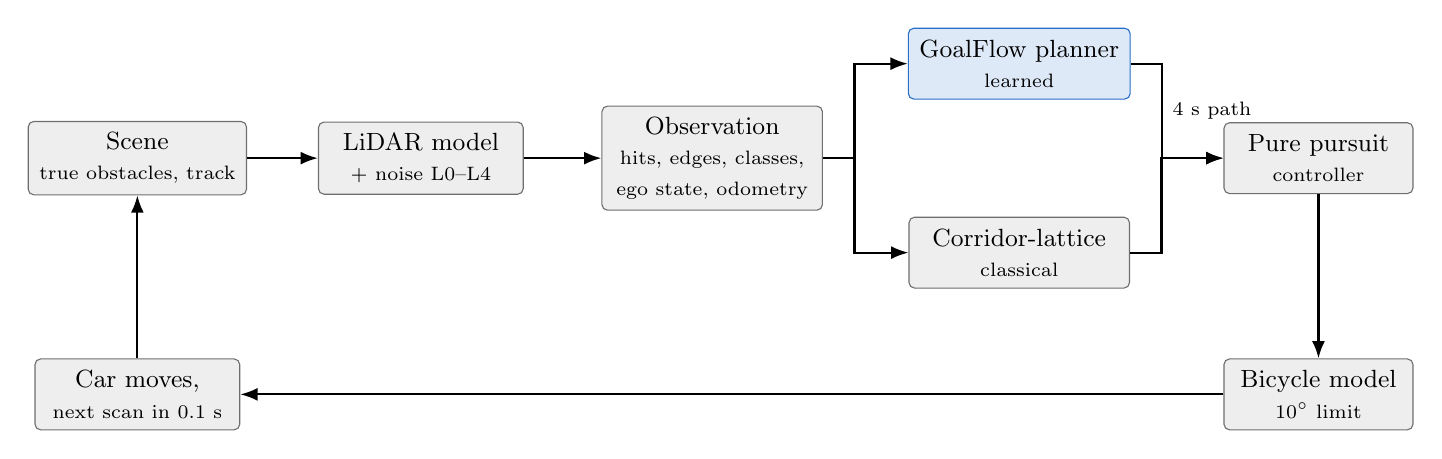
\begin{tikzpicture}
  \node[classic, minimum width=26mm] (scene) at (0,0) {Scene\\\scriptsize true obstacles, track};
  \node[classic, minimum width=26mm] (lidar) at (3.6,0) {LiDAR model\\\scriptsize + noise L0--L4};
  \node[classic, minimum width=28mm] (obs) at (7.3,0) {Observation\\\scriptsize hits, edges, classes,\\\scriptsize ego state, odometry};
  \node[learned, minimum width=28mm] (gf) at (11.2,1.2) {GoalFlow planner\\\scriptsize learned};
  \node[classic, minimum width=28mm] (cl) at (11.2,-1.2) {Corridor-lattice\\\scriptsize classical};
  \node[classic, minimum width=24mm] (pp) at (15,0) {Pure pursuit\\\scriptsize controller};
  \node[classic, minimum width=24mm] (bike) at (15,-3) {Bicycle model\\\scriptsize $10^\circ$ limit};
  \node[classic, minimum width=26mm] (move) at (0,-3) {Car moves,\\\scriptsize next scan in 0.1 s};
  \draw[arr] (scene) -- (lidar);
  \draw[arr] (lidar) -- (obs);
  \draw[arr] (obs.east) -- ++(4mm,0) |- (gf.west);
  \draw[arr] (obs.east) -- ++(4mm,0) |- (cl.west);
  \draw[arr] (gf.east) -- ++(4mm,0) |- node[pos=0.25,right,font=\scriptsize]{4 s path} (pp.west);
  \draw[arr] (cl.east) -- ++(4mm,0) |- (pp.west);
  \draw[arr] (pp) -- (bike);
  \draw[arr] (bike) -- (move);
  \draw[arr] (move) -- (scene);
\end{tikzpicture}}
\caption{The closed loop. Every 0.1\,s the simulated LiDAR produces a noisy observation, a planner returns
a 4\,s path, and the same controller and vehicle model drive it. Blue = learned, grey = classical.}
\label{fig:loop}
\end{figure}

\subsection{Teacher and student}
The project uses a \term{teacher--student} setup:
\begin{itemize}[nosep]
  \item The \term{teacher} is the classical corridor-lattice planner given the \emph{true} scene (exact
        obstacles and edges). It plans once at the start and drives the course.
  \item The \term{student}, GoalFlow, sees only the noisy LiDAR picture and learns to imitate the teacher.
  \item The \term{observed baseline} is the same classical planner running on the noisy LiDAR picture.
\end{itemize}
This makes the comparison fair: GoalFlow and the classical baseline receive exactly the same information.

\subsection{The four planners compared}
\begin{table}[h]
\small
\begin{tabularx}{\linewidth}{@{}lLL@{}}
\toprule
Planner & Sees & Role \\
\midrule
Teacher (privileged corridor-lattice) & true scene & reference behaviour, training targets, feasibility \\
Observed corridor-lattice & noisy LiDAR & main classical baseline (configs a--d) \\
Regression & BEV image & learned baseline: one network outputs one path \\
GoalFlow & BEV image & the method under test \\
\bottomrule
\end{tabularx}
\end{table}

\subsection{What GoalFlow sees: the bird's-eye-view (BEV) image}
The observation is turned into a $6\times128\times128$ image covering 25.6\,m around the car at 0.2\,m per
cell (\code{sim/raster.py}). The six layers are: LiDAR hits, free space (cells crossed by LiDAR rays),
unknown (never reached), drivable area (between the observed track edges), obstacle class (bollard or
cone, from the camera), and the goal direction. This mirrors the costmap that Nav2 builds on the real car,
so the same interface can later be fed from CARLA or from Juno.

%=====================================================================
\section{The simulator and the training data}
%=====================================================================

\subsection{Scenes and seeds}
Each scene (track shape plus obstacle layout) is generated from an integer \term{seed}. Seeds 0--499 are
the development set for closed-loop evaluation. Training, validation and test scenes use separate seed
ranges (100000+, 200000+, 300000+; the spent test split is 300000+, the fresh test set will be
400000+). Of seeds 0--499, 477 scenes are feasible; in the other 23 no gap passes
the door rule and the correct behaviour is to stop.

\subsection{Unseen edges}
Where the LiDAR does not see a track edge, the planners guess it from the opposite edge shifted by 12\,m
(the \term{fill}), using a curve fit before offsetting.

\subsection{How training data is made}
\label{sec:data}
The teacher drives each training scene in closed loop while the simulated LiDAR records. A frame is saved
at 5\,Hz with the observation and one or more 4\,s target paths (\term{modes}):
\begin{enumerate}[nosep]
  \item \textbf{Mode 0} is the path the teacher actually drove next.
  \item \textbf{Alternatives}: every 10 frames the teacher is rerun from the current state to find up to
        $K=8$ distinct routes through the obstacles; between reruns they are re-tracked from the car's pose
        and dropped if more than 0.5\,m away.
  \item \textbf{Deduplication by homotopy}: for each path we record on which side it passes every obstacle
        within 3\,m of the path (distance to its nearest point; obstacles nearest its first or last pose are
        ignored); paths with the same signature count once. Each mode is therefore a genuinely
        different way past the obstacles.
  \item \textbf{Recovery frames} (27\%): the car is placed up to 1\,m sideways and $15^\circ$ off, and the
        target is a fresh teacher plan, so the model learns to recover from mistakes.
\end{enumerate}
The training set has about 658{,}000 frames, with a noise mix of 15/25/25/20/15\% for L0--L4.

%=====================================================================
\section{The classical planner: corridor-lattice}
\label{sec:classical}
%=====================================================================

\begin{enumerate}[nosep]
  \item \textbf{Obstacle fitting}: LiDAR hits are clustered; each cluster becomes a circle whose radius
        comes from its class (bollard/cone) and whose centre is fitted.
  \item \textbf{Gaps}: the obstacle centres and track edges are connected by a \term{Delaunay
        triangulation}; each triangle edge between two obstacles is a ``door'', kept if it passes the
        door rule.
  \item \textbf{Routes}: \term{A*} search over the triangles finds the best few routes to the goal line.
  \item \textbf{Path}: inside each route's corridor, a \term{lattice search} over forward arcs finds a path
        the car can steer, trying curvature limits of 0.8, 0.9 and 0.95 of $\kappa_{\max}$.
  \item \textbf{Margins}: plans keep 0.25\,m clearance; a path being followed is accepted down to 0.12\,m.
\end{enumerate}

\paragraph{Configurations.} (a) the original planner plus a goal-line fix; (b) (a) plus the \emph{L3
additions}: obstacle tracking, edge memory, plan hysteresis with fallback, hold after a brake, and a
failed-search cache; (c) (b) without edge memory; (d) (b) without tracking. Section~\ref{sec:results}
gives their results.

%=====================================================================
\section{GoalFlow: how it works and where it happens}
%=====================================================================

\begin{figure}[h]
\centering
\resizebox{\linewidth}{!}{%
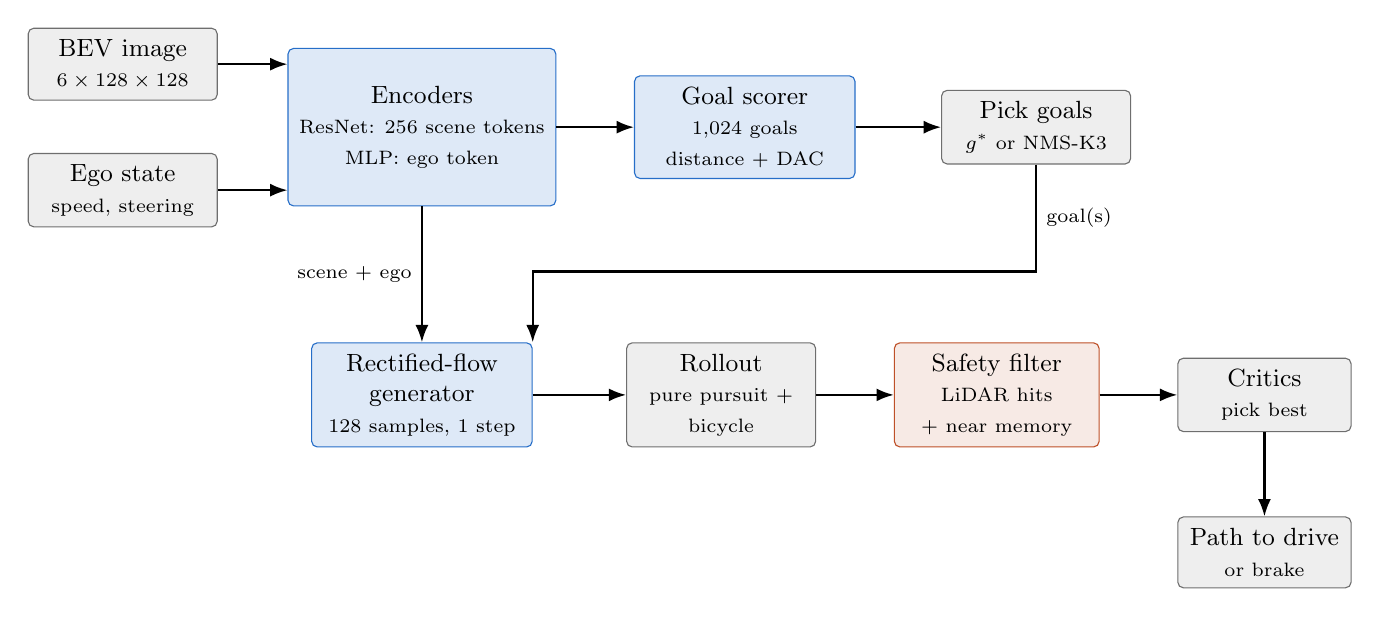
\begin{tikzpicture}
  \node[classic, minimum width=24mm] (bev) at (0,0.8) {BEV image\\\scriptsize $6\times128\times128$};
  \node[classic, minimum width=24mm] (ego) at (0,-0.8) {Ego state\\\scriptsize speed, steering};
  \node[learned, minimum width=30mm, minimum height=20mm] (enc) at (3.8,0) {Encoders\\\scriptsize ResNet: 256 scene tokens\\\scriptsize MLP: ego token};
  \node[learned, minimum width=28mm] (gs) at (7.9,0) {Goal scorer\\\scriptsize 1{,}024 goals\\\scriptsize distance + DAC};
  \node[classic, minimum width=24mm] (sel) at (11.6,0) {Pick goals\\\scriptsize $g^*$ or NMS-K3};
  \node[learned, minimum width=28mm] (flow) at (3.8,-3.4) {Rectified-flow\\generator\\\scriptsize 128 samples, 1 step};
  \node[classic, minimum width=24mm] (roll) at (7.6,-3.4) {Rollout\\\scriptsize pure pursuit +\\\scriptsize bicycle};
  \node[safety, minimum width=26mm] (safe) at (11.1,-3.4) {Safety filter\\\scriptsize LiDAR hits\\\scriptsize + near memory};
  \node[classic, minimum width=22mm] (crit) at (14.5,-3.4) {Critics\\\scriptsize pick best};
  \node[classic, minimum width=22mm] (out) at (14.5,-5.4) {Path to drive\\\scriptsize or brake};
  \draw[arr] (bev) -- (bev -| enc.west);
  \draw[arr] (ego) -- (ego -| enc.west);
  \draw[arr] (enc) -- (gs);
  \draw[arr] (gs) -- (sel);
  \draw[arr] (enc) -- node[left,font=\scriptsize]{scene + ego} (flow);
  \draw[arr] (sel.south) |- node[pos=0.25,right,font=\scriptsize]{goal(s)} ($(flow.north east)+(0,0.9)$) -- ($(flow.north east)+(0,0)$);
  \draw[arr] (flow) -- (roll);
  \draw[arr] (roll) -- (safe);
  \draw[arr] (safe) -- (crit);
  \draw[arr] (crit) -- (out);
\end{tikzpicture}}
\caption{GoalFlow inside one planning step (\code{GoalFlow.plan()} in \code{models/goalflow.py}).
Blue = neural networks, grey = fixed rules, red = hard geometric safety check.}
\label{fig:gf}
\end{figure}

GoalFlow happens in two places. The neural network and the per-frame decision live in
\code{src/gfsem/models/goalflow.py} (method \code{plan()}). The closed-loop wrapper that calls it every
0.1\,s, keeps the obstacle memory and brakes when nothing is safe is
\code{src/gfsem/planners/goalflow\_planner.py}. The model has 10.1\,M parameters in total.

\subsection{Step 1: see (perception encoder)}
A small \term{ResNet} (\code{encoders.py}) reduces the $128\times128$ BEV image in three stride-2 stages to
a $16\times16$ grid of features, projected to 256 dimensions. With a 2D sine/cosine position code added,
this gives 256 \term{tokens}, each describing a $1.6\times1.6$\,m patch of the scene. A small MLP encodes
the ego state (speed, steering) into one more vector.

\subsection{Step 2: decide where to go (goal vocabulary and scorer)}
\paragraph{Vocabulary.} A fixed list of 1{,}024 candidate end points, each with position and heading, was
built by \term{k-means clustering} over the end points of all teacher routes in the training data. It
covers 0--12\,m ahead and about $\pm6.6$\,m sideways; every teacher route ends within 0.5\,m of some goal.

\paragraph{Scorer.} Each goal becomes a query vector (an MLP over a sinusoidal encoding of $(x,y,\theta)$,
plus the ego vector). Three \term{cross-attention} layers let every query look at the 256 scene tokens.
Two small heads then output, per goal:
\begin{itemize}[nosep]
  \item a \term{distance score}: how close the goal is to where the teacher would end up;
  \item a \term{DAC score} (drivable area compliance): the probability that the car parked at that goal
        would be inside the track and clear of every obstacle.
\end{itemize}
The final score is $\log \mathrm{softmax}(\text{distance}) + \log \sigma(\text{DAC})$. The best goal is
called $g^*$.

\paragraph{NMS-K (our extension).} Instead of sending all samples to $g^*$, we take the best goal and then
the next best goals that lie at least 1.5\,m from those already chosen (non-maximum suppression), up to
$K=3$. The 128 samples are split across these goals. This turned out to be the key improvement
(Section~\ref{sec:results}).

\subsection{Step 3: generate paths (rectified flow)}
The generator (\code{flow\_generator.py}) is a transformer. Its input tokens are: 16 environment tokens
(learned queries that cross-attend to the scene tokens), one goal token, 16 waypoint tokens (the current
noisy path), and one time token. Four transformer layers process them, and the network outputs a
\term{velocity} for each waypoint. Starting from random noise, one step along this velocity turns noise
into a 4\,s path that heads for the goal. Section~\ref{sec:ml} explains rectified flow.

\subsection{Step 4: make paths drivable (rollout)}
Every sampled path is fed to a simulated pure-pursuit controller (2.5\,m lookahead) driving a kinematic
bicycle model with the real limits ($10^\circ$ steering, $40^\circ$/s steering rate, 1\,m/s$^2$
acceleration, 3\,m/s$^2$ braking), for 80 steps of 0.05\,s (\code{rollout.py}). The result, the
\term{executed path}, is what the car would actually drive. All later checks use it.

\subsection{Step 5: remove unsafe paths (safety filter)}
A distance transform of the LiDAR-hit layer gives, for every cell, the distance to the nearest hit. The
car's footprint is covered by $8\times4$ small circles (radius 0.231\,m) placed along each executed path
every 0.2\,m. A path is rejected if any circle comes closer to a hit than its radius. The filter uses only
what the sensor saw (plus a short memory, Section~\ref{sec:evade}), never the true scene. If no path
survives, the planner brakes.

\subsection{Step 6: choose (critics)}
The surviving paths are scored by
\[
  f = -\lambda_1\,\widehat{d}_{\text{goal}} + \lambda_2\,\widehat{p}_{\text{progress}} + \lambda_4\,\widehat{s}_{\text{goal}},
  \qquad (\lambda_1,\lambda_2,\lambda_4) = (1,\,0.5,\,1),
\]
where $\widehat{\cdot}$ means rescaled to $[0,1]$ over the candidates: the distance from the path's end to
its own goal, the forward progress, and the score of the goal it was aimed at. A consistency term with the
previous plan exists ($\lambda_3$) but is off. The best path is driven.

\subsection{The shadow path (off)}
The paper also samples paths with no goal at all and switches to the best of them when it differs a lot
from the chosen path. In our tests it added collisions and bypassed the safety filter, so it is off.

\subsection{Training}
The model is trained in three stages (encoder and goal scorer, then the generator, plus the regression
baseline); Section~\ref{sec:training} explains them in detail.

%=====================================================================
\section{Training in detail}
\label{sec:training}
%=====================================================================

Training has two parts: building the data from the teacher, and training the network in three stages.
Code: \code{src/gfsem/train.py}; overnight settings: \code{scripts/launch\_full\_training.sh}.

\subsection{The data the network learns from}
\begin{itemize}
  \item \textbf{Frames.} About 6{,}000 training scenes driven by the teacher give about 658{,}000 frames at
        5\,Hz. Each frame stores the raw observation (hits, rays, edges, classes, ego state), up to 8
        teacher routes of 16 poses, the scene seed and the true pose.
  \item \textbf{Rasterised on the fly.} The 6-channel BEV image is built from the stored observation when the
        frame is loaded. This keeps the dataset within a 20\,GB budget and lets the rasteriser change without
        regenerating data.
  \item \textbf{Target route.} One of the frame's teacher routes is drawn at random as this step's target.
  \item \textbf{DAC labels} for all 1{,}024 goals are computed at load time from the true scene: place the car's
        footprint at each goal and test it against the track and every obstacle.
  \item \textbf{Normalisation.} Path coordinates are mapped per axis to about $[-1,1]$ using the 1st and 99th
        percentiles of the training paths.
  \item \textbf{Built-in augmentation.} 27\% recovery frames (car moved up to 1\,m sideways, $15^\circ$ off,
        target = fresh teacher plan) counter imitation learning's blind spot, and the noise mix
        (L0 15\%, L1 25\%, L2 25\%, L3 20\%, L4 15\%) teaches robustness.
  \item \textbf{Splits} use disjoint seed ranges; a fixed random subset of 4{,}000 validation frames is used
        during training.
\end{itemize}

\subsection{Before training: the goal vocabulary (unsupervised)}
All teacher-route end points $(x,y,\theta)$ are clustered with k-means into 1{,}024 clusters (heading
weighted so that 1\,rad counts as 2\,m; k-means++ initialisation, 30 refinement rounds, up to 200{,}000
points). The cluster centres become the vocabulary (\code{vocab.npy}); it is fixed and never trained.

\subsection{Stage A: perception and goal scorer}
\textit{Trains} the ResNet encoder, the ego encoder and the goal scorer; \textit{learns} to read the scene
and rank goals.
\begin{itemize}
  \item \textbf{Distance head: cross-entropy with soft targets.} For the teacher's end point
        $g_{\text{teacher}}$, each vocabulary goal gets a target probability
        $q_i \propto \exp(-\lVert g_i - g_{\text{teacher}}\rVert / 0.5\,\mathrm{m})$, so nearby goals share
        the credit. The loss is
        \[ L_{\text{dis}} = -\sum_i q_i \log \mathrm{softmax}(s)_i . \]
        It cannot reach zero: its minimum is the entropy of $q$ (about 5.5), which mostly explains the plateau (the remaining gap is about 0.3)
        near 5.8 seen during training.
  \item \textbf{DAC head: binary cross-entropy} per goal against the drivable labels;
        $L_A = L_{\text{dis}} + 0.1\,L_{\text{DAC}}$ in the overnight run.
  \item Batch 64, computed as two half-batches of 32 whose gradients are summed (gradient accumulation) to
        fit the Mac's memory; 3-hour budget; 12{,}784 steps.
\end{itemize}

\subsection{Stage B: the path generator (rectified flow)}
\textit{Trains} only the generator. Stage A is frozen, including its BatchNorm statistics, so the scene
features do not drift. Each step:
\begin{enumerate}[nosep]
  \item take the normalised target path $x_1$ and noise $x_0\sim\mathcal{N}(0,0.1^2 I)$;
  \item draw $t\in[0,1]$ uniformly and form $x_t=(1-t)\,x_0+t\,x_1$;
  \item the generator sees $x_t$, $t$, the scene and the goal (the target path's real end point) and
        predicts a velocity;
  \item loss: $L_{\text{flow}} = \lvert v_\theta - (x_1-x_0)\rvert$ (L1).
\end{enumerate}
\begin{itemize}
  \item \textbf{One step at inference.} Because the learned paths from noise to data are straight lines,
        one Euler step suffices: path $= x_0 + v_\theta(x_0, 0)$.
  \item \textbf{Goal dropout.} In 10\% of examples the goal is replaced by a learned null token, so the same
        network can also generate without a goal (the shadow path; same idea as classifier-free guidance in
        image diffusion).
  \item \textbf{Real end point vs vocabulary goal.} Training conditions on the true end point; inference
        uses vocabulary goals. This works because the vocabulary covers every route end within about 2\,cm
        (median).
  \item Batch 64, 3.5-hour budget, 86{,}603 steps (cheap steps, since the encoder is frozen).
\end{itemize}

\subsection{Regression baseline}
A separate encoder plus a head of 16 learned queries that attend to the scene and output 16 waypoints
directly; L1 loss to the target path; 1.5-hour budget, 15{,}875 steps. Trained on the same random route per
frame, it can learn the \emph{average} of left and right where both exist (mode averaging). Open loop it
collides in 3.2\% of frames, against 0.79\% for single-goal GoalFlow and 0.36\% for the chosen configuration.
Its rate is about the same in single-route and multi-route frames (3.0\% vs 3.2\%), so mode averaging is not
the only cause: it is also less precise in general.

\subsection{Optimisation settings (all stages)}
\begin{table}[h]
\small
\begin{tabularx}{\linewidth}{@{}lLL@{}}
\toprule
Setting & Value & Why \\
\midrule
Optimiser & AdamW, learning rate $3\times10^{-4}$, weight decay 0.01 & standard for transformers \\
Schedule & 50 warm-up steps, then cosine decay to 0 & stable start, gentle finish \\
Gradient clipping & global norm 1.0 & prevents occasional huge updates \\
Precision & fp32 on the Mac; mixed precision only on CUDA & fp16 on Apple MPS is unreliable \\
Time budget & after 60 steps, measure seconds per step and set the total so the stage fits its budget & the overnight run ends on time \\
\bottomrule
\end{tabularx}
\end{table}

\subsection{Choosing checkpoints and stopping}
\begin{itemize}[nosep]
  \item Validation every 30 minutes on the 4{,}000-frame subset.
  \item The kept checkpoint (\code{*\_best.pt}) is chosen by: stage A, lowest validation goal loss (switched
        mid-run from goal error, which stopped improving while everything else improved); stage B and
        regression, lowest ADE of the \emph{executed} path against the driven teacher route.
  \item Early stopping after 4 evaluations without improvement (never triggered).
  \item The full training state is saved every 30 minutes, so an interrupted run resumes mid-stage.
\end{itemize}

\subsection{Known weaknesses and plans}
\begin{enumerate}[nosep]
  \item \textbf{Mixture target} (implemented behind a flag): train the distance head on the average of all
        the frame's route targets in one step, instead of one random route. This also steadies the stage-A
        validation metric, which wobbled because the drawn route changed between evaluations.
  \item \textbf{The driven route dominates}: mode 0 is in every frame, alternatives in about 11\%, so the
        scorer ranks the driven route first. The mixture target should lift the second route.
  \item \textbf{Stage B stopped while still improving} (smoothness was still getting better).
  \item \textbf{Only one seed.} Seeds 1--2 are needed to know how much results vary between training runs
        (Colab Pro or the Bylogix GPUs).
  \item \textbf{Imitation sets the ceiling.} GoalFlow copies the teacher, including its conservative door
        rule; it can beat the classical baseline only through better use of noisy perception and multiple
        routes, not by driving better than the teacher.
\end{enumerate}

%=====================================================================
\section{How we evade obstacles}
\label{sec:evade}
%=====================================================================

Obstacle avoidance is not one component but several layers, from soft preferences learned by the network
to a hard geometric veto. If all layers fail to find a safe path, the car brakes.

\begin{figure}[h]
\centering
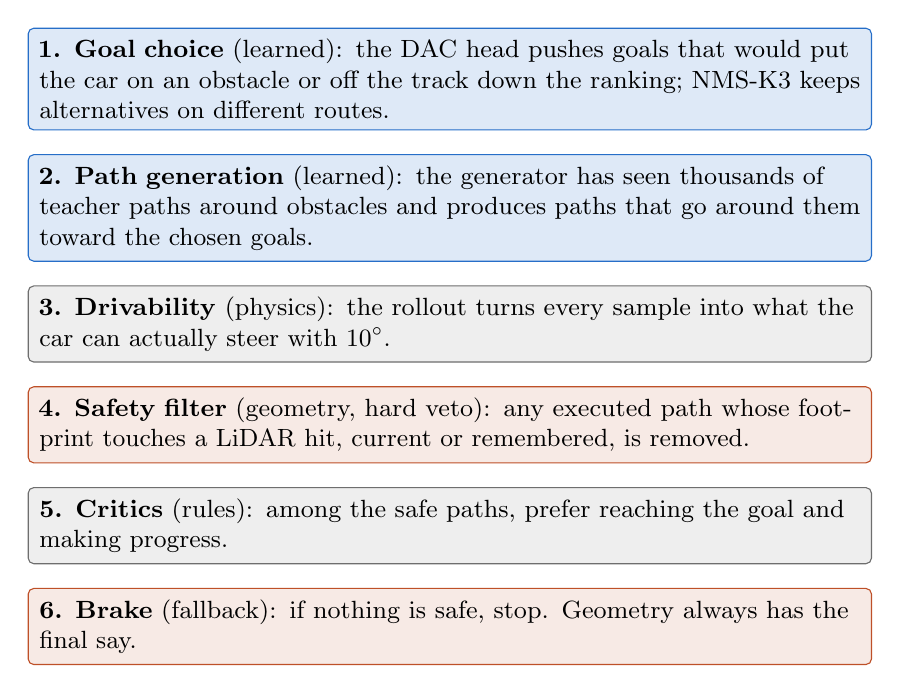
\begin{tikzpicture}[node distance=3mm]
  \node[learned, text width=0.86\linewidth, align=left] (l1) {\textbf{1. Goal choice} (learned): the DAC head pushes goals that would put the car on an obstacle or off the track down the ranking; NMS-K3 keeps alternatives on different routes.};
  \node[learned, below=of l1, text width=0.86\linewidth, align=left] (l2) {\textbf{2. Path generation} (learned): the generator has seen thousands of teacher paths around obstacles and produces paths that go around them toward the chosen goals.};
  \node[classic, below=of l2, text width=0.86\linewidth, align=left] (l3) {\textbf{3. Drivability} (physics): the rollout turns every sample into what the car can actually steer with $10^\circ$.};
  \node[safety, below=of l3, text width=0.86\linewidth, align=left] (l4) {\textbf{4. Safety filter} (geometry, hard veto): any executed path whose footprint touches a LiDAR hit, current or remembered, is removed.};
  \node[classic, below=of l4, text width=0.86\linewidth, align=left] (l5) {\textbf{5. Critics} (rules): among the safe paths, prefer reaching the goal and making progress.};
  \node[safety, below=of l5, text width=0.86\linewidth, align=left] (l6) {\textbf{6. Brake} (fallback): if nothing is safe, stop. Geometry always has the final say.};
\end{tikzpicture}
\caption{The layers of obstacle avoidance in GoalFlow.}
\end{figure}

\subsection{Why a memory is needed near the car}
The LiDAR cannot see everything close to Juno. With the sensor at the front axle, the 1.5\,m blind zone
reaches about 0.86\,m past the front bumper. Worse, the lowest beam points $19^\circ$ below horizontal, so
a 0.40\,m cone passes under it once it is within about 2.03\,m of the sensor. Planning from a single scan,
GoalFlow ``forgot'' cones right before reaching them, and every collision in early tests was of this kind.

We therefore give the safety filter (only the filter; the network input stays single-scan) a short memory
of LiDAR hits:
\begin{itemize}[nosep]
  \item only hits observed within 4\,m of the sensor are remembered (far observations are distorted by
        odometry drift when mapped back: up to 1\,m in our tests);
  \item a 0.2\,m cell counts only after it was hit in at least two scans (removes single-scan clutter);
  \item cells are stored in the car's own, drifting odometry frame, never the true pose, and are kept
        until they are behind the rear bumper or more than 4\,m away.
\end{itemize}
Four memory designs were compared under a rule fixed in advance; this one removed all collisions in the
smoke test without adding stalls.

\subsection{How the classical planner avoids obstacles}
The corridor-lattice planner avoids obstacles by construction: it only plans through gaps that pass the
door rule and only accepts paths with 0.25\,m clearance (0.12\,m while following). Keeping its previous
plan gives it an implicit memory of obstacles it no longer sees.

%=====================================================================
\section{The machine-learning and AI methods, explained}
\label{sec:ml}
%=====================================================================

\subsection{Learning paradigms}
\begin{description}[style=nextline,leftmargin=0pt]
  \item[Supervised learning] Learning a function from examples with known answers (inputs and labels).
        The DAC head is supervised: its labels (drivable or not) are computed from the true scene.
  \item[Imitation learning / teacher--student] A special case of supervised learning where the labels are
        an expert's actions. Our expert is the privileged planner; GoalFlow learns to produce its paths from
        noisy input. Recovery frames counter the classic weakness of imitation (never seeing its own
        mistakes).
  \item[Unsupervised learning] Finding structure without labels. The goal vocabulary is built with
        \textbf{k-means}, which groups 200{,}000 route end points into 1{,}024 clusters and keeps their
        centres.
  \item[Self-supervised learning] Learning from data that labels itself. In the earlier video phase we used
        \textbf{DINOv2}, a vision transformer pretrained this way, as a frozen feature extractor (23\,ms on the
        Orin, drivable-area IoU 0.954 with a linear probe).
\end{description}

\subsection{Network building blocks}
\begin{description}[style=nextline,leftmargin=0pt]
  \item[Convolutional neural network (CNN) and ResNet] A CNN slides small learned filters over an image to
        detect local patterns; stacking them builds up larger patterns. A ResNet adds ``skip connections'' so
        each block learns a correction to its input, which makes deeper networks train reliably. Our BEV
        encoder is a small ResNet.
  \item[Multilayer perceptron (MLP)] A few fully connected layers; used to embed the ego state, goals and time.
  \item[Transformer and attention] Attention lets each token compute a weighted average of other tokens,
        with weights learned from how relevant they are. \emph{Self-attention}: tokens attend to each other.
        \emph{Cross-attention}: one set of tokens (queries, e.g.\ goals) attends to another (the scene).
        Transformers stack attention and MLP layers. Both the goal scorer and the generator are transformers.
  \item[Sinusoidal encoding] Numbers such as coordinates or time are turned into sines and cosines at many
        frequencies, so the network can represent fine and coarse variations.
\end{description}

\subsection{Generative models: diffusion, flow matching, rectified flow}
A \term{generative model} learns a distribution and can draw new samples from it; here, the distribution of
good paths given the scene and a goal. This matters because there are often several good answers (left or
right of an obstacle).
\begin{description}[style=nextline,leftmargin=0pt]
  \item[Diffusion models] Learn to reverse a process that gradually adds noise to data. Sampling starts from
        pure noise and removes it step by step (often tens of steps).
  \item[Flow matching] Learns a \emph{velocity field} that moves samples from noise to data along a
        continuous path; sampling integrates this field.
  \item[Rectified flow] Flow matching with straight-line paths. For a training path $x_1$ and noise
        $x_0\sim\mathcal{N}(0,\sigma^2 I)$ ($\sigma=0.1$), take a random $t\in[0,1]$ and the point
        $x_t=(1-t)\,x_0+t\,x_1$; the network learns the constant velocity $v=x_1-x_0$:
        \[
          \mathcal{L} = \bigl\lVert v_\theta(x_t,t,\text{scene},\text{goal}) - (x_1-x_0)\bigr\rVert_1 .
        \]
        Because the paths are straight, very few integration steps are needed; we use one step,
        $\hat{x}_1 = x_0 + v_\theta(x_0,0,\dots)$. Two or four steps make raw paths smoother but did not change
        the driven paths.
  \item[Why not plain regression?] A \textbf{regression} network outputs one path that minimises average
        error. When half the examples go left and half go right, the average goes straight, often into the
        obstacle (\term{mode averaging}). Our regression baseline collides in 3.2\% of frames open loop,
        about 4 times single-goal GoalFlow (0.79\%) and 9 times the chosen configuration (0.36\%). Its rate is
        similar in single- and multi-route frames, so averaging is one cause among others.
\end{description}

\subsection{Losses}
\begin{description}[style=nextline,leftmargin=0pt]
  \item[Cross-entropy with soft targets] Used for the distance head: the target is a probability spread over
        goals near the teacher's end point (temperature 0.5\,m), and the loss is lowest when the predicted
        distribution matches it. Its minimum is the target's entropy, which mostly explains the training plateau.
  \item[Binary cross-entropy] Used for the DAC head: a yes/no prediction per goal.
  \item[L1 loss] Used for the flow velocity: the average absolute difference.
\end{description}

\subsection{Classical AI, planning and control}
\begin{description}[style=nextline,leftmargin=0pt]
  \item[Delaunay triangulation] Connects points into triangles with no point inside any triangle's
        circumcircle; gives the natural ``doors'' between obstacles.
  \item[A* search] Finds the cheapest path in a graph, guided by an estimate of the remaining cost.
  \item[Lattice planning] Searches over a fixed set of drivable motion pieces (arcs), so every result
        respects the turning limit.
  \item[MPPI] Model Predictive Path Integral control: samples many perturbed control sequences, simulates
        them, and averages them weighted by cost. GoalFlow is similar in spirit (sample, simulate, score);
        using a GoalFlow path as the starting point for MPPI is queued to make paths more precise in tight gaps.
  \item[Pure pursuit] A steering law that aims at a point a fixed distance (2.5\,m) ahead on the path.
  \item[Kinematic bicycle model] A simple car model: two wheels on a line, front one steering; enough to
        capture the turning limit at low speed.
  \item[Homotopy] Two paths are in the same homotopy class if they pass every obstacle on the same side;
        it is our formal notion of ``a different route''.
\end{description}

\subsection{Statistics}
\begin{description}[style=nextline,leftmargin=0pt]
  \item[Paired comparison and McNemar's test] Variants are evaluated on the same frames. McNemar's test
        looks only at frames where exactly one variant fails and asks whether that split could be chance.
\end{description}

%=====================================================================
\section{How we measure}
%=====================================================================

\begin{table}[h]
\small
\begin{tabularx}{\linewidth}{@{}lL@{}}
\toprule
Metric & Meaning \\
\midrule
Success (closed loop) & reaches the goal line without collision or track exit; \% of the 477 feasible scenes \\
Collision & the car's footprint overlaps a true obstacle (open loop: the 4\,s plan of one frame) \\
Stall & the car stops and never reaches the goal \\
ADE / FDE & average / final distance between a path and the teacher's path (describes imitation, not quality) \\
DAC accuracy & how often the DAC head is right about a goal being drivable \\
cover@$k$ & the $k$ best candidates include one near every teacher route \\
Homotopy cover & a path passes every obstacle on the same side as a teacher route \\
\bottomrule
\end{tabularx}
\end{table}

\textbf{Open loop} checks one frame's plan without driving it; \textbf{closed loop} drives the whole
course with the planner in control. Safety and progress metrics decide; ADE and FDE only describe.

%=====================================================================
\section{Results so far}
\label{sec:results}
%=====================================================================

\subsection{Goal scorer (validation, 66{,}063 frames)}
The scorer sees both routes around an obstacle: the driven route ranks first, and once near-duplicate goals
are skipped the other route is the second pick in 76\% of cases and in the top five in 96.5\%. The early
impression that it only predicted one route came from an unsuitable metric. The real weakness was that all
samples were sent to one goal.

\subsection{Selection variants (open loop, 11{,}331 validation frames)}
\begin{table}[h]
\small
\begin{tabularx}{\linewidth}{@{}Lrr@{}}
\toprule
Variant & Collisions & Brakes \\
\midrule
Regression & 3.17\% & -- \\
GoalFlow, single goal (as in the paper; no filter) & 0.79\% & -- \\
GoalFlow, NMS-K3 + safety filter, shadow on & 0.59\% & 0.54\% \\
\textbf{GoalFlow, NMS-K3 + safety filter, shadow off (chosen)} & \textbf{0.36\%} & \textbf{0.54\%} \\
Classical planner, single scan & 0.07\% & 3.8\% \\
\bottomrule
\end{tabularx}
\end{table}
Three goals plus the safety filter is the real gain (paired McNemar $p=0.004$; main path $p\approx2\times10^{-8}$).
With a single goal the filter does nothing: all samples follow nearly the same line, so there is no safe
alternative to switch to.

\subsection{Classical baseline (closed loop, seeds 0--499; success \%)}
\begin{table}[h]
\small
\begin{tabular}{@{}lrrrrr@{}}
\toprule
Config & L0 & L1 & L2 & L3 & L4 \\
\midrule
Before fixes & 91.2 & 97.1 & 98.1 & 94.8 & 70.0 \\
(a) original + goal-line fix & 94.8 & 97.1 & 97.1 & \textbf{96.6} & \textbf{93.7} \\
(b) + L3 additions & 97.5 & 97.3 & 95.8 & 92.5 & 74.8 \\
(c) (b) without edge memory & 95.4 & 96.9 & 94.3 & 89.5 & 77.1 \\
(d) (b) without tracking & \textbf{97.9} & \textbf{97.5} & 94.8 & 74.4 & 37.1 \\
\bottomrule
\end{tabular}
\end{table}
Two edge-handling bugs were found and fixed (an edge stub at the goal line and an edge guess inside the real
edge). The L3 additions help at low noise but stall at high noise: their obstacle tracker turns LiDAR clutter
into about five phantom obstacles per scan at L4, and the ``hold'' rule waits for confirmations that noisy
scans rarely give. GoalFlow is compared against the best configuration at each level: (a) at L2--L4, (b) at
L0--L1, with (c) also reported.

\subsection{Closed-loop GoalFlow (smoke test, seeds 0--39)}
\begin{table}[h]
\small
\begin{tabular}{@{}lcc@{}}
\toprule
Planner & L0 (success/coll./stall/exit) & L4 (success/coll./stall/exit) \\
\midrule
GoalFlow, near-field memory & 37 / 0 / 2 / 0 & 35 / 0 / 4 / 0 \\
Classical (a) & 37 / 0 / 0 / 2 & 35 / 1 / 3 / 0 \\
Classical (b) & 39 / 0 / 0 / 0 & 31 / 1 / 7 / 0 \\
\bottomrule
\end{tabular}
\end{table}
On 39 feasible scenes per level this is indicative only. GoalFlow had no collisions; ``no safe candidate''
brakes happened in 3.0\% of planning steps. All six GoalFlow failures are stalls in scenes where baseline (a)
succeeds: GoalFlow's candidates pass very close to obstacles in tight gaps (in seed 17 the best candidate
cleared by a median 1\,cm), so the safety filter rejects them all and the car brakes. In seed 1 at L0 the
opposite happened: (a) left the track and GoalFlow succeeded. Refining the chosen GoalFlow path with MPPI is
queued to fix the precision problem. The full run (500 seeds, all levels) is next. Planning takes about
183\,ms per step on the Mac; the 50\,ms Orin target is not yet met.

%=====================================================================
\section{Lessons for the real car}
%=====================================================================
\begin{itemize}[nosep]
  \item \textbf{Remember nearby obstacles.} Cones vanish under the lowest beam within about 2\,m of the
        sensor; Nav2's obstacle layer must keep them and must not clear cells there.
  \item \textbf{Keep that memory short-range.} Odometry drift distorts far observations; the ZED odometry
        read 10--60\% low in our recordings.
  \item \textbf{Mounting matters.} Moving the EMX further back shrinks the blind area past the bumper.
  \item \textbf{Respect the turning limit.} Use Nav2 Smac Hybrid-A* or State Lattice with a 9.1\,m minimum
        radius, not a funnel plus pure pursuit.
  \item \textbf{Two margins.} Plan with 0.25\,m clearance, accept down to 0.12\,m while following.
  \item \textbf{Trackers need a birth rule.} A track should exist only after several consistent sightings.
\end{itemize}

%=====================================================================
\section{Open problems and next steps}
%=====================================================================
\begin{enumerate}[nosep]
  \item Full closed-loop GoalFlow run: 500 seeds $\times$ L0--L4 (Mac or chunked on Colab Pro).
  \item Precision in tight gaps: refine the chosen GoalFlow path with MPPI.
  \item Tracker birth rule and duplicate merging; then a tracked-perception GoalFlow variant.
  \item A plan should only be accepted if its end state allows a way on (dead ends in the classical planner).
  \item Latency on the Orin; a deterministic per-step search budget for the classical planner.
  \item Retraining with a mixture target and more seeds (Colab Pro or the Bylogix GPUs), CARLA transfer.
  \item Final numbers on the fresh test set (seeds 400000+).
\end{enumerate}

\appendix
\section{Glossary}
\begin{description}[style=nextline,leftmargin=0pt,nosep]
  \item[BEV] Bird's-eye view: a top-down image of the surroundings.
  \item[DAC] Drivable area compliance: whether a goal pose is inside the track and clear of obstacles.
  \item[Door rule] The minimum gap the car may pass through: $\text{gap}-2r\ge 1.165+0.5$\,m.
  \item[$g^*$] The best-scored goal.
  \item[Homotopy class] The set of paths passing every obstacle on the same side.
  \item[L0--L4] LiDAR noise levels, from perfect to very noisy.
  \item[Mode] One stored teacher route for a frame.
  \item[NMS-K] Picking the $K$ best goals at least 1.5\,m apart.
  \item[Oracle / teacher] The classical planner with access to the true scene.
  \item[Open / closed loop] Checking one plan vs driving the whole course with the planner.
  \item[Rectified flow] A generative model that learns straight-line velocities from noise to data.
  \item[Rollout] Simulating how the car would drive a path.
  \item[Safety filter] The geometric check that removes paths touching LiDAR hits.
\end{description}

\end{document}
